\clearpage


\section{等待 ALOHA 的提出及分析}

\subsection{系统模型}

本方案考虑一个包含一个接入点（Access Point，AP）和 $N$ 个设备的无线网络，各个设备采纳时隙 ALOHA 的方式接入网络并进行网络传输。如图\ref{fig:system_model}所示。
\begin{figure}[h]
    \centering
    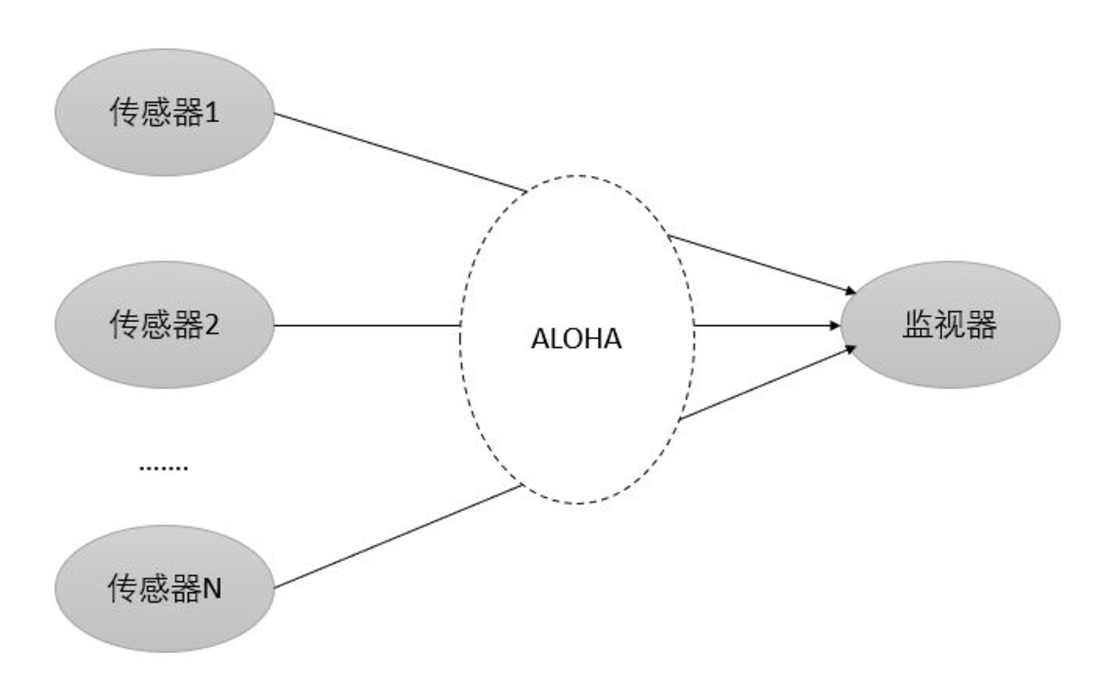
\includegraphics[width=0.8\textwidth]{figure/cp3/系统模型图.pdf}
    \caption{系统模型图}
    \label{fig:system_model}
\end{figure}

在经典的时隙 ALOHA 协议中，时间被划分为等长的离散系统时隙。为实现状态更新，各节点在生成数据包后，统一于每个时隙的起始边界以固定概率 $p_0$ 接入信道并尝试传输。鉴于该机制缺乏载波侦听功能，为缓解多节点并行传输导致的信道碰撞，系统引入了退避机制：发生传输失败的节点需初始化一个退避计数器。随着系统时隙的推进，该计数器逐时隙递减，当计数器归零时，节点才能再次接入信道。在上述介质访问控制的基础上，本文引入了\textbf{按需生成}采样策略。与传统的排队缓冲机制不同，在按需生成的策略下，节点不再维护数据包队列以存储历史数据，而是采取“即发即采”的原则。具体而言，节点仅在决定发起传输的瞬间，才即时对底层物理过程进行采样，并生成全新的状态更新包。这一策略消除了数据包在发送端的排队延迟，根据 AoI 的定义，网络中任意节点在离散系统时隙 $t$ 中的 AoI 演化方程可具体表示为：
\begin{equation}
    \label{eq:aoi_evolution}
    \Delta(t+1) = 
    \begin{cases} 
        1, & \text{若设备在时隙 } t \text{ 成功传输了数据包} \\ 
        \Delta(t) + 1, & \text{其他情况（传输失败或退避中）}
    \end{cases}
\end{equation}

在节点数量较少、网络负载较轻的环境下，传统时隙 ALOHA 模型凭借其极简的协议架构、极低的信令开销以及易于分布式部署的特性，展现出了极高的工程实用价值。它无需依赖复杂的中心化调度，即可低成本地满足设备间基本的数据连通需求。然而，它并不适用于海量设备接入的大规模物联网中。在这种场景下，以传感器生成的传感数据为例，传感数据一般用来描述所观测物理现象的最新状态，而接收端需要这些数据来感知周边物理环境，以做出最佳决策。在这种需求下，单个设备的连续且紧挨着的数据传输并不能带来显著增益，因为接收端已经掌握了发送端的最新状态。相反，长时间未成功传输的设备，接收端对其所掌握的状态信息已经严重老化，亟需优先接入信道以完成状态更新。因此，从全局优化的网络视角来看，各个设备不应拘泥于自私的盲目竞争，而应以“协同”的方式接入信道。刚刚完成状态更新的设备理应让出信道资源，为那些尚未完成更新的设备提供更多的传输机会。为此，我们将基于等待的随机接入机制引入时隙 ALOHA，构建等待 ALOHA 协议，该机制的核心规则如下：

\textbf{在每次成功传输后，协议强制该设备主动退避$z$个时隙}。这里的 $z$ 是一个常数等待窗口，用于迫使刚成功更新的设备在接下来的 $z$ 个系统时隙内不参与信道的竞争。这一等待窗口为其他未更新的设备提供了更多的传输机会。

\textbf{在每次传输失败后，碰撞设备将根据$\beta \sim \text{unif}(0,w-1)$生成新的退避计时器}。通过保留时隙 ALOHA 的退避机制，可有效降低拥塞环境下的碰撞概率。

根据所提协议，节点在每个系统时隙的退避计时器变化关系如下：
\begin{equation}
    b_i(t + 1) =
\begin{cases}
z, & \text{if } b_i(t) = 0, \, b_j(t) \neq 0 \ \forall j, \\
\beta, & \text{if } b_i(t) = 0, \, b_j(t) = 0 \ \exists j, \\
b_i(t) - 1, & \text{if } b_i(t) \neq 0.
\end{cases}
\end{equation}
式中，$b_j(t)$ 表示除 $i$ 以外的节点的退避计时器状态。在此系统模型下，节点的 AoI 演化轨迹如同锯齿波波形，如图\ref{fig:cp3_aoi_evolution}所示。在接收端未收到节点的更新数据包时，AoI 将随时间线性增长；当接收到更新数据包时，AoI 下降到 1。
\begin{figure}[h]
\centering
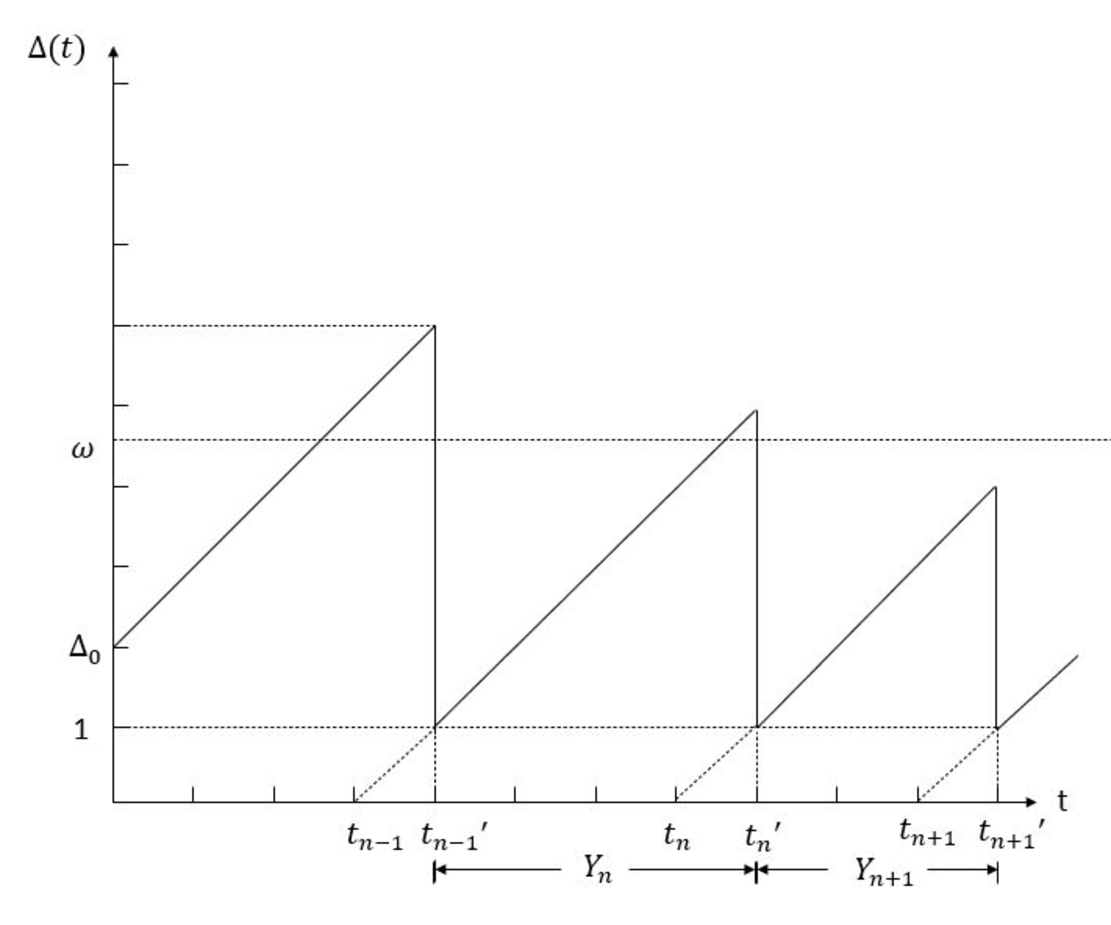
\includegraphics[width=0.8\textwidth]{figure/cp3/AoI变化趋势图.pdf}
\caption{AoI变化趋势图}
\label{fig:cp3_aoi_evolution}
\end{figure}

正如第二章所推导的通用计算公式所示，评估系统平均 AoI 及 AoI 违规概率的核心，在于求解离开时间间隔 $Y$ 的一阶矩与二阶矩 。为了实现这一理论推导目标，最直观的数学手段是利用马尔可夫链对系统状态进行精确建模。然而，若构建一个联合涵盖所有设备 AoI、退避计时器及设备总数量的马尔可夫链，随着网络规模 $N$ 的增长，系统的状态空间将发生指数级的维度增长，导致方程极度复杂且难以解析求解。为克服这一理论推导瓶颈，本文借鉴了 Bianchi 模型中处理强耦合演化过程的经典解耦方法，引入如下近似假设：当网络规模相对较大时，系统迅速趋于平稳，可认为在任意系统时隙中，单一节点的碰撞概率 $p_{cl}$ 是一个不受时间影响的独立常数。这一近似假设的物理合理性在于：当某一目标源尝试发送数据包时，网络中其他节点的退避计数器已经收敛至相同的稳态概率分布。因此，无论在哪个时隙进行传输，目标节点的系统争用环境始终是一个恒定的状态。在包含大量节点的实际状态更新系统中，这种近似已被证明具有极高的精确度。基于此解耦假设，我们能够将高维系统降维，仅仅通过追踪一个单一目标节点的马尔可夫状态演化，即可完成对系统性能指标的严谨分析。

\subsection{基于马尔可夫链的稳态接入分析}

在等待 ALOHA 中，数据包能否成功交付，直接受制于网络中多节点并发引发的碰撞概率 $p_{cl}$。因此，求解 $p_{cl}$ 是贯穿整个协议理论分析的关键。基于前面引入的解耦假设，本小节将构建目标节点的离散时间马尔可夫链模型，通过联立节点的稳态发送概率与系统全局的碰撞概率，建立描述系统模型的稳态方程，并严格论证其稳态解的存在性与唯一性。

\subsubsection{状态转移模型}

为了捕捉节点在等待 ALOHA 机制下的微观行为，设目标节点在时隙 $t$ 的状态定义为 $(m(t),n(t))$，其中 $m(t)$ 表示节点当前时隙的退避计时器数值，$n(t)$ 表示节点当前时隙的 AoI。记
\begin{equation}
    b_{i,k}=\lim_{t \to +\infty} \text{Pr}\{m(t)=i,n(t)=k\}
\end{equation}
为系统状态的平稳分布。

依据等待 ALOHA 的运行机制，当退避计时器大于0时，节点不参与信道的竞争，所以在经过一个时隙后，退避计时器会减少1，而 AoI 则会增加1。只有当设备的退避计时器等于0时，设备才会被唤醒，并出现以下三种动作：
\begin{enumerate}[wide]
    \item 不发送数据包，退避计时器保持0，AoI 增加1，即 $(0,k)\to(0,k+1)$，显然，转移概率为 $1-p_0$；
    \item 尝试发送数据包，但是发生了碰撞，此时 AoI 增加1，退避计时器在 $[0,w-1]$ 的区间内随机选择，即 $(0,k)\to(i,k+1),i\in[0,w-1]$，转移概率为 $q=\frac{p_{cl}}{w}$；
    \item 成功发送数据包，此时 AoI 置为1，退避计时器置为 $z$，即 $(0,k)\to(z,1)$，转移概率为 $p_s=p_0(1-p_{cl})$。
\end{enumerate}

由于成功传输的设备会主动退避 $z$ 个时隙，进入 $(z,1)$ 状态。在接下来的 $z$ 个时隙，退避计时器会依次减1，AoI 则会依次加1，直到退避计时器等于0，此时 AoI 将等于 $z+1$，即有着 $(z,1)\to(z-1,2)\to(z-2,3)\to\cdots\to(1,z)\to(0,z+1)$ 的确定性状态跃迁链。因此，当系统处于稳态运行时，能够再次发包的首个活跃状态为 $(0,z+1)$。基于上述转移规则，我们可以绘制出完整的二维马尔可夫链，如图\ref{fig:cp3_aloha_system_tran_photo}所示。其中，为了简记，记 $p=(1-p_0)+\frac{p_0p_{cl}}{w}$，$\omega$为预设的 AoI 门限。
\begin{figure}[h]
    \centering
    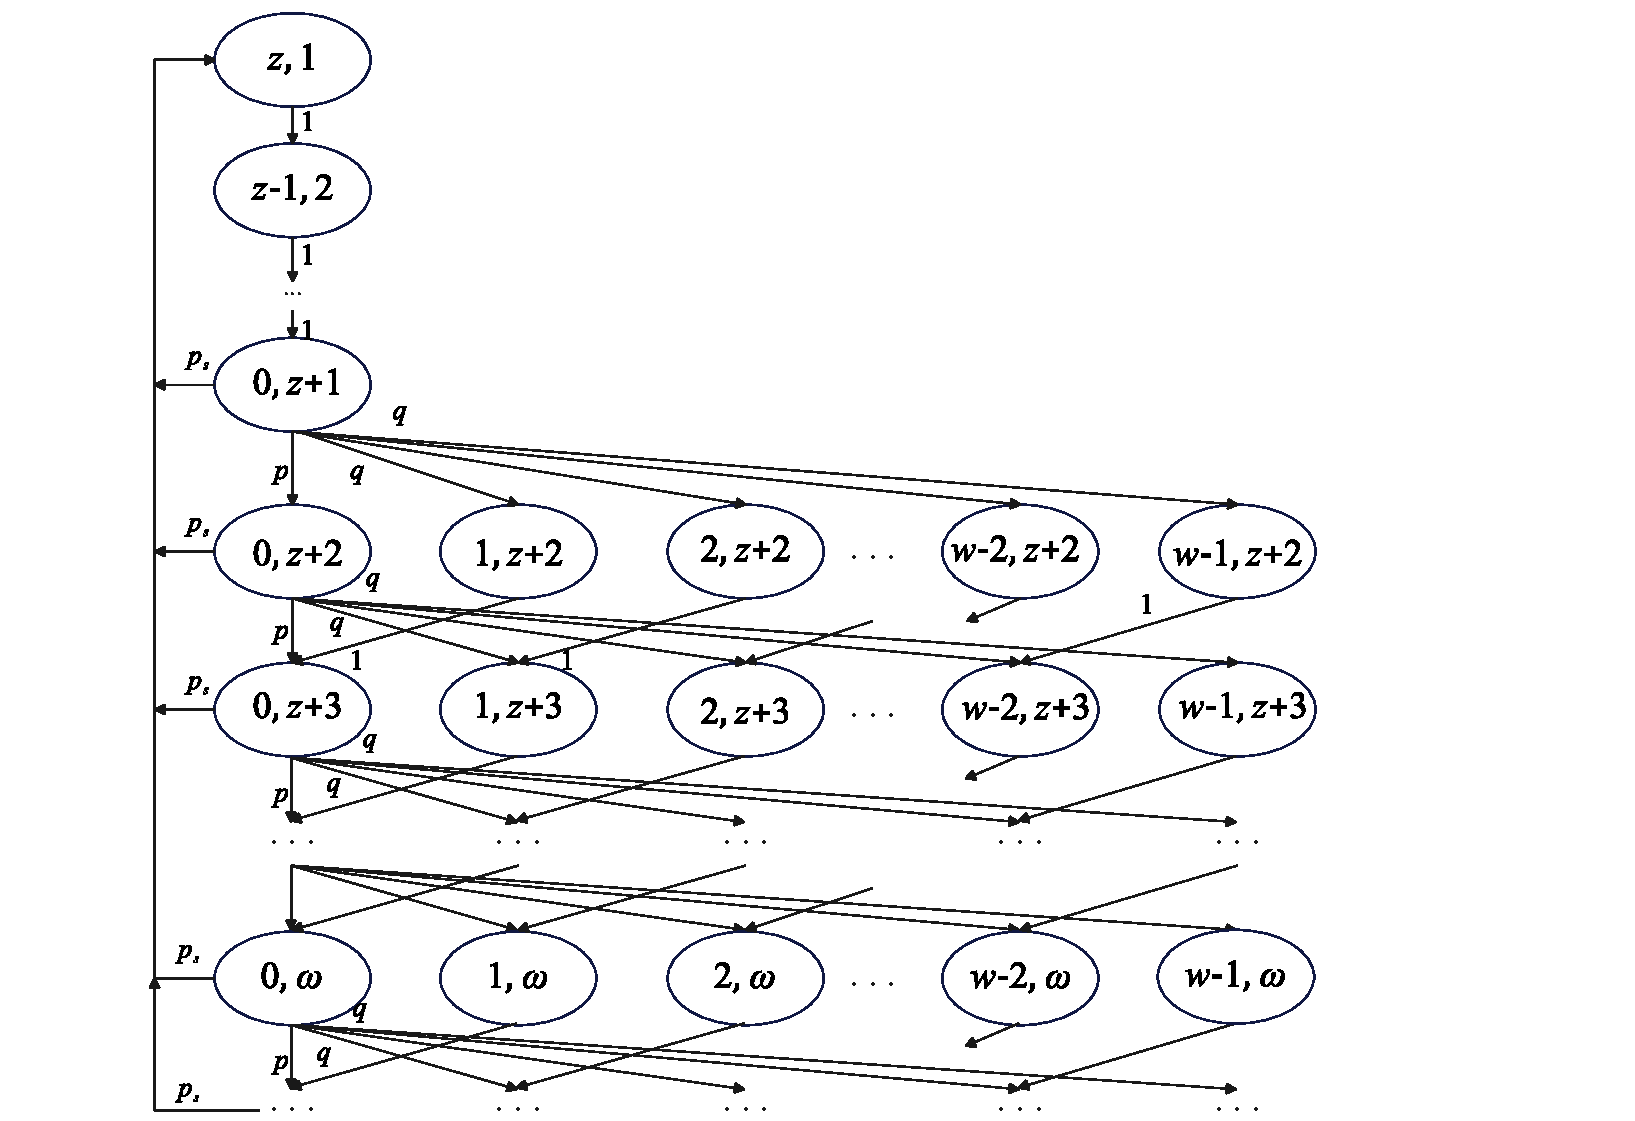
\includegraphics[width=0.8\textwidth]{figure/cp3/系统的状态转移图.pdf}
    \caption{系统的状态转移图}
    \label{fig:cp3_aloha_system_tran_photo}
\end{figure}

\subsubsection{稳态方程的构建}

观察图\ref{fig:cp3_aloha_system_tran_photo}，发现处于任意状态 $(i,k)$ 的平稳概率 $b_{i,k}$ 均可溯源并表示为若干个活跃状态概率 $b_{0,m}$ 的线性组合。当 AoI 不大于 $z+1$ 时，
\begin{equation} \label{cp3_b_ik_aoi_le_z+1}
    b_{z,1}=b_{z-1,2}=b_{z-2,3}=\cdots=b_{0,z+1}=p_s\sum_{k=z+1}^{+\infty}b_{0,k}
\end{equation}
当 AoI 等于 $z+2$ 时，
\begin{equation}\label{cp3_b_ik_equal_z+2}
    b_{0,z+2} = pb_{0,z+1},b_{i,z+2}=qb_{0,z+1},\quad1\leq i \leq w-1
\end{equation}
当 AoI 大于 $z+2$ 时，对于任意的 $m$，$n$，都有
\begin{equation}\label{cp3_b_ik_great_z+2}
\begin{gathered}
\begin{cases} 
    % 第1行
    \displaystyle b_{0,n} = p b_{0,n-1} + q \sum_{k=z+1}^{n-2} b_{0,k}, & z+3 \le n \le z+w+1 \\[20pt]
    
    % 第2行
    \displaystyle b_{0,n} = p b_{0,n-1} + q \sum_{k=n-w}^{n-2} b_{0,k}, & n > z+w+1 \\[20pt]
    
    % 第3行
    \displaystyle b_{m,n} = q \sum_{k=z+1}^{n-1} b_{0,k}, & m \ge 1, m+n \le z+w+1 \\[20pt]
    
    % 第4行
    \displaystyle b_{m,n} = q \sum_{k=m+n-w}^{n-1} b_{0,k}, & m \ge 1, m+n > z+w+1
\end{cases}
\end{gathered}
\end{equation}
根据概率的归一化性质，将式\eqref{cp3_b_ik_aoi_le_z+1}，\eqref{cp3_b_ik_equal_z+2}，\eqref{cp3_b_ik_great_z+2}联立起来，可得：
\begin{equation}
\begin{split}
(z+1)p_0(1-p_{cl}) \sum_{k=z+1}^{\infty} b_{0,k} + (1-p_0) \sum_{k=z+1}^{\infty} b_{0,k} \\
+ p_0 p_{cl} \sum_{k=z+1}^{\infty} b_{0,k} + \frac{p_0 p_{cl}(w-1)}{2} \sum_{k=z+1}^{\infty} b_{0,k} = 1
\end{split}
\end{equation}
对上式进行整理，最终得到：
\begin{equation}\label{cp3_sum_of_b_0k}
\sum_{k=z+1}^{\infty} b_{0,k} = \frac{1}{1 + z p_0 - z p_0 p_{cl} + \frac{p_0 p_{cl} w}{2} - \frac{p_0 p_{cl}}{2}}
\end{equation}
对式\eqref{cp3_sum_of_b_0k}进行观察，可知右侧的求和结果仅依赖于系统的稳态碰撞概率 $p_{cl}$。

在此系统模型下，目标节点在任意一个给定时隙向无线信道发起传输的平均发送概率 $\tau$ 等于其恰好处于退避计时器等于0的状态且自身决定发送的联合概率。因此，平均发送概率与碰撞概率的关系如下：
\begin{equation}\label{cp3_avg_send_prob}
    \tau=p_0\sum_{k=z+1}^{+\infty}b_{0,k}=\frac{p_0}{1+zp_0+p_0p_{cl}(\frac{w-1}{2}-z)}=\tau(p_{cl})
\end{equation}

另一方面，在包含 $N$ 个活跃节点的网络中，由于各个节点的发送行为被假设为相互独立，因此目标节点在某次尝试发送时遭遇碰撞的概率 $p_{cl}$ 等于网络中至少存在另外一个节点在同一时隙内发送数据包的概率，这一概率可表述如下：
\begin{equation}\label{cp3_pcl_with_tau}
    p_{cl} = 1- (1-\tau)^{N-1}
\end{equation}

将\eqref{cp3_avg_send_prob}代入\eqref{cp3_pcl_with_tau}，可以消去中间变量$\tau$，得到一个只包含未知数$p_{cl}$的稳态自洽方程：
\begin{equation}\label{cp3_pcl}
    p_{cl} = 1 - (1 - \tau(p_{cl}))^{N-1} \triangleq f(p_{cl})
\end{equation}

\subsubsection{稳态方程解的存在唯一性论证}

从数学性质上看，方程\eqref{cp3_pcl}是一个高阶的非线性方程，无法通过常规的代数变换方法来获得闭式解，因此考虑使用数值迭代的方法来进行求解。在使用数值迭代的方法之前，需要解决两个问题：一是这个方程在定义域 $[0,1]$ 内是否存在解，二是这个解是否具有唯一性。

构造辅助函数 $F(x) = x - f(x)$，有 $F(0)=0-f(0)<0$，$F(1)=1-f(1)>0$，因此如果能够证明 $F(x)$ 单调递增，就能够保证方程 $F(x)=0$ 在区间 $[0,1]$ 上有唯一解。对 $F(x)$进行求导，可以得到
\begin{equation}
    F'(x)=1-f'(x)=1-(N-1)(1-\tau(x))^{N-2}\frac{p_0^2(\frac{w-1}{2}-z)}{[D(x)]^2}
\end{equation}
其中，$D(x)=1+zp_0+p_0p_{cl}(\frac{w-1}{2}-z)$。

为了确保理论推导的鲁棒性，此次论证选取系统最为敏感的饱和临界负载状态，即总网络负载 $G = N\tau \approx 1$ 进行渐近分析。在该极限条件下，指数衰减项 $(1-\frac{1}{N})^{N-2}$ 并未趋近于0，而是收敛于 $\frac{1}{e}$。此时，$f'(x)$ 的量级将完全被线性项 $(N-1)$ 所主导 。

根据 $w$ 与 $z$ 的取值不同， $F'(x)$ 将呈现出不同的结果,下面分情况进行讨论： 
\begin{enumerate} [wide]
    \item 假设 $\frac{w-1}{2}\ge z$，即 $w \ge 2z+1$，此时 $f'(x) < 0$，可以得到 $F'(x)>0$，证明了 $F(x)$ 是一个单调递增的函数，因此 $F(x)$ 在区间 $[0,1]$ 上有唯一解。
    \item 假设$\frac{w-1}{2} < z$，即 $w<2z+1$，此时 $f'(x) > 0$，$f(x)$ 是递增的，如果能够证明 $f'(x) \le 1$，那么就可保证$F(x)=0$在区间$[0,1]$上的唯一性。然而，随着网络规模 $N$ 的增大，$f'(x)$将增长并突破1的界限，这意味着在$\frac{w-1}{2} < z$的条件下无法保证$f'(x)\le1$恒成立，也就无法保证$F(x)=0$在区间$[0,1]$上的唯一性。
\end{enumerate}  

综上，当 $w \ge 2z+1$ 时，稳态方程\eqref{cp3_pcl}有唯一解，其为等待 ALOHA 的理论边界约束。在此约束下，用于快速求解稳态解的不动点迭代算法步骤如下：
\begin{enumerate}[wide]
    \item \textbf{初始化：}设定迭代轮次计数器 $t=0$，在 $(0,1)$ 区间内选取任意合理初始值 $p_{cl}^{(0)}$，并设定极小的收敛容差阈值 $\epsilon$。
    \item \textbf{状态更新：}依据当前轮次的碰撞概率，计算节点的平均发送概率 $\tau(p_{cl}^{(t)})$，随后依据非线性映射关系刷新碰撞概率估计值：$p_{cl}^{(t+1)} = 1 - \big(1 - \tau(p_{cl}^{(t)})\big)^{N-1}$。
    \item \textbf{收敛判定：}持续追踪前后两次迭代差值的绝对值 $|p_{cl}^{(t+1)} - p_{cl}^{(t)}|$。若该差值缩小至 $\epsilon$ 以内，则算法成功收敛，输出的极限值 $p_{cl}^*$ 即为网络真实的稳态碰撞概率；否则自增迭代次数继续演化。
\end{enumerate}

根据此法求得的碰撞概率 $p_{cl}^*$，将作为已知系统常量，直接用于后续 AoI 指标的计算之中。

\subsection{信息时效性指标的理论解析}
\subsubsection{平均 AoI 的闭式推导}

在第二章中，我们分析得到了平均 AoI 的通用计算公式 \eqref{cp2_avg_aoi}，由于在此系统模型下，系统时间$T$恒等于1，因此平均 AoI 可使用下式计算：
\begin{equation}\label{cp3_avg_aoi}
    \Delta = 1 + \frac{E[Y^2]}{2E[Y]}
\end{equation}
式中，$Y$ 表示离开时间间隔。分析式\eqref{cp3_avg_aoi}的形式，可知求解平均AoI的关键在于得到 $Y$ 的一阶矩与二阶矩，因此下面将对 $Y$ 的前两阶矩进行推导。

\begin{enumerate}[wide]
    \item 求解 $Y$ 的一阶矩 
    
    假设在 $Y$ 内总共发起了 $\alpha$ 次数据包的传输，由于在解耦假设下，每次传输的碰撞概率 $p_{cl}$ 为一独立常数，因此传输次数 $\alpha$ 服从参数为 $1-p_{cl}$ 的几何分布，其概率质量函数为：
    \begin{equation}\label{cp3_alpha_expression}
        Pr\{\alpha=k\}=(1-p_{cl})*p_{cl}^{k-1},k=1,2,\dots
    \end{equation}

    根据等待 ALOHA 的设计规则，一次完整的离开时间间隔 $Y$ 总共包含三个部分。第一部分是节点每次成功传输后，主动退避的 $z$ 个系统时隙。第二部分是节点每次尝试传输所耗费的系统时隙，记这部分时隙为 $I$，其概率质量函数为：
    \begin{equation}\label{cp3_I_expression}
        Pr\{I=i\}=(1-p_0)^{i-1}*p_0
    \end{equation}

    第三部分是节点每次碰撞后，在 $[0,w-1]$ 内随机选择一个退避计时器 $\beta$。将这些部分合计起来，可得到 $Y_k$ 的表达式：
    \begin{equation}\label{cp3_Yk_expression}
        Y_k=z+\sum_{j=1}^{k-1}(I_j+\beta_j)+I_{k}=z+\sum_{j=1}^{k}I_j+\sum_{j=1}^{k-1}\beta_j
    \end{equation}

    每一个 $I_j$ 与 $\beta_j$ 都是互相独立的，且除 $Y_k$ 以外的随机变量都服从标准分布，在\cite{probability_book}中可直接得到它们对应的期望，因此 $Y_k$ 的一阶矩为：
    \begin{equation}\label{cp3_EYk}
        E[Y_k]=z+\frac{k}{p_0}+\frac{(k-1)(w-1)}{2}
    \end{equation}

    联立式\eqref{cp3_alpha_expression}和式\eqref{cp3_EYk}，可以得到 $Y$ 的期望值如下：
    \begin{equation}\label{cp3_EY}
        \begin{split}
            E[Y] &= \sum_{k=1}^{+\infty}\Pr\{\alpha=k\}E[Y_k] \\
            &= z\sum_{k=1}^{+\infty}(1-p_{cl})p_{cl}^{k-1} + \frac{1}{p_0}\sum_{k=1}^{+\infty}k(1-p_{cl})p_{cl}^{k-1} \\
            &\quad + \frac{w-1}{2}\sum_{k=1}^{+\infty}(k-1)(1-p_{cl})p_{cl}^{k-1} \\
            &= z + \frac{1}{p_0(1-p_{cl})} + \frac{p_{cl}(w-1)}{2(1-p_{cl})}
        \end{split}
    \end{equation}
    上式中包含了几何分布的零阶矩与一阶矩的求和形式，可在\cite{probability_book}中查找得到。

    \item 求解 $Y$ 的二阶矩
    
    根据方差的定义，对于给定的传输次数 $\alpha=k$ ，随机变量 $Y_k$ 的二阶矩可以表示为：
    \begin{equation}\label{cp3_EYk^2}
        E[Y_k^2] = D(Y_k) + (E[Y_k])^2
    \end{equation}

    根据方差的线性性质，常数 $z$ 的方差为0，由于 $I_j$ 与 $\beta_j$ 相互独立，因此 $Y_k$ 的方差可表示为：
    \begin{equation}\label{cp3_DYk}
        D(Y_k) = \sum_{j=1}^{k} D(I_j) + \sum_{j=1}^{k-1} D(\beta_j) = k D(I) + (k-1) D(\beta)
    \end{equation}

    联立式\eqref{cp3_DYk}，式\eqref{cp3_EYk}与式\eqref{cp3_EYk^2}，可得到 $E[Y_k^2]$ 的表达式：
    \begin{equation}\label{cp3_EYK^2_withAB}
        \begin{aligned}
            E[Y_k^2] &= k \frac{1-p_0}{p_0^2} + (k-1)\frac{w^2-1}{12} + (U + kV)^2 \\
            &= \left( U^2 - \frac{w^2-1}{12} \right) + k \left[ \frac{1-p_0}{p_0^2} + \frac{w^2-1}{12} + 2UV \right] + k^2 V^2
        \end{aligned}
    \end{equation}
    式中，$U=Z-\frac{w-1}{2}$，$V=\frac{1}{p_0}+\frac{w-1}{2}$。

    联立式\eqref{cp3_alpha_expression}和式\eqref{cp3_EYK^2_withAB}，可得到 $Y$ 的二阶矩形式：
    \begin{equation}\label{cp3_EY2}
        \begin{aligned}
            E[Y^2] &= \sum_{k=1}^{+\infty} \Pr\{\alpha=k\} E[Y_k^2] \\
            &= \left( U^2 - \frac{w^2-1}{12} \right) \sum_{k=1}^{+\infty}(1-p_{cl})p_{cl}^{k-1} \\
            &\quad + \left[ 2UV + \frac{1-p_0}{p_0^2} + \frac{w^2-1}{12} \right] \sum_{k=1}^{+\infty} k(1-p_{cl})p_{cl}^{k-1} \\
            &\quad + V^2 \sum_{k=1}^{+\infty} k^2(1-p_{cl})p_{cl}^{k-1}
        \end{aligned}
    \end{equation}
    对上式进行整理，得到 $E[Y^2]$ 的最终表达式：
    \begin{equation}\label{cp3_EY2result}
        E[Y^2] = z^2 + \left[ \frac{2 + p_{cl} p_0 (w-1)}{p_0 (1-p_{cl})} \right] z + C_0
    \end{equation}
    式中，$C_0$ 展开整理如下：
    \begin{equation*}
        \begin{split}
            C_0 &= \frac{1}{(1-p_{cl})^2} \Bigg\{ \frac{p_{cl}(p_{cl}+2)}{6} w^2 - \frac{p_{cl} [ p_0(1+p_{cl}) - 4 ]}{2 p_0} w \\
                &\quad + \frac{p_{cl}(2p_{cl}+1)}{6} - \frac{p_{cl}+1}{p_0} + \frac{2}{p_0^2} \Bigg\}
        \end{split}
    \end{equation*}
\end{enumerate}

最后，联立式\eqref{cp3_EY}，式\eqref{cp3_EY2result}与式\eqref{cp3_avg_aoi}，可得到平均 AoI 的闭式表达式：
\begin{equation}\label{cp3_AoI_Final}
    \begin{aligned}
        \Delta = 1 + \frac{z^2 + \left[ \frac{2 + p_{cl} p_0 (w-1)}{p_0 (1-p_{cl})} \right] z + C_0}{2 \left[ z + \frac{1}{p_0(1-p_{cl})} + \frac{p_{cl}(w-1)}{2(1-p_{cl})} \right]}
    \end{aligned}
\end{equation}


\subsubsection{AoI 违规概率的闭式推导}
图\ref{fig:cp3_aoi_evolution_with limit}是带有阈值 $\omega$ 的AoI演化图，在第二章 AoI 违规概率的计算公式已由\eqref{cp2_aoi_violation_expression}给出，其中分母 $E[Y]$ 的闭式已经得到，因此求解违规概率的关键在于得到违规量的期望 $E[J]$，即 $E[max(0,1+Y-\omega)]$。$\omega$ 是 AoI 的阈值。为了求解 $E[J]$，接下来将求解出 $Y$ 的概率密度函数 $f_Y(y)$。
\begin{figure}[h]
    \centering
    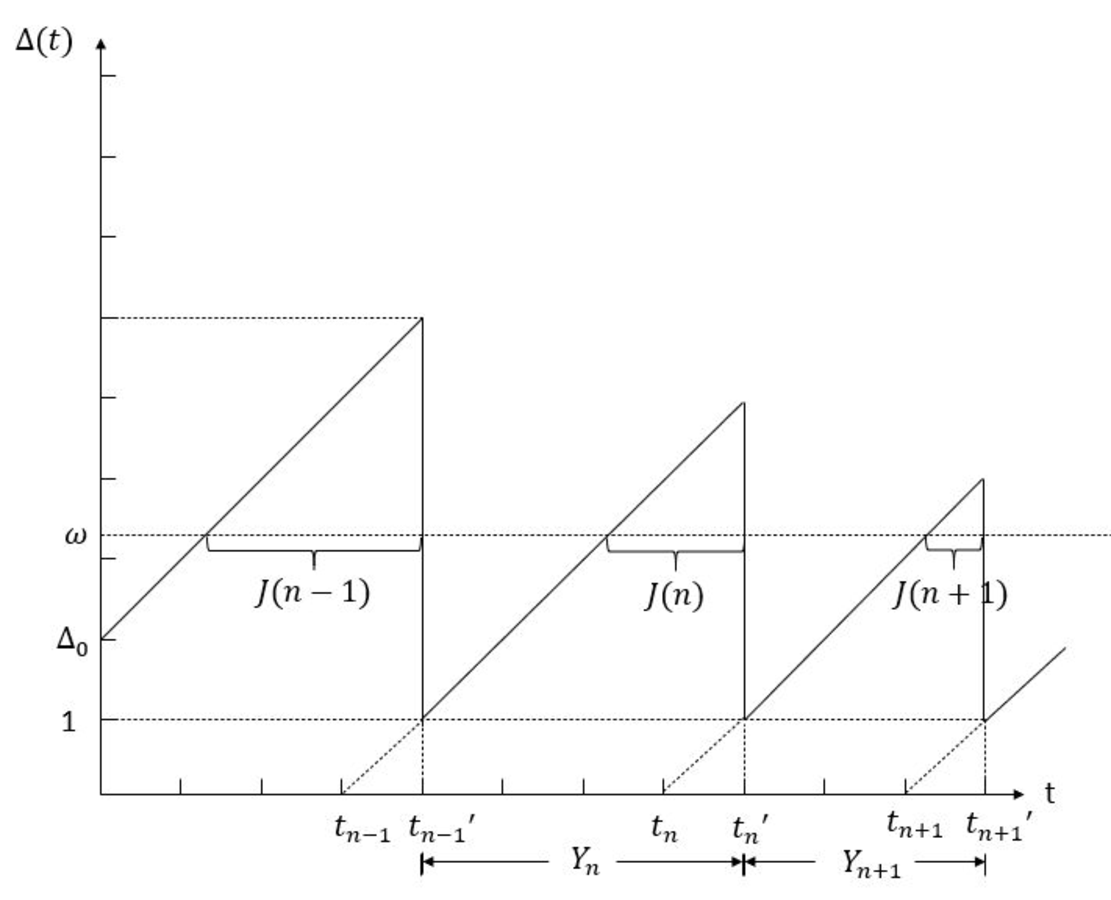
\includegraphics[width=0.8\textwidth]{figure/cp3/有限制的AoI演化图.pdf}
    \caption{具有$\omega$限制的AoI演化图}
    \label{fig:cp3_aoi_evolution_with limit}
\end{figure}

从系统演化的微观过程来看，$Y$ 是由随机个服从几何分布的传输尝试与服从均匀分布的退避时隙累加而成，尽管理论上可以通过几何分布和均匀分布的卷积推导出 $Y$ 的精确概率密度函数，但整个过程将十分复杂，且最终得到的表达式将是一个包含多项式分段函数的无穷级数，计算复杂度极高，难以应用于实际分析。

针对于难以直接求解 $f_Y(y)$ 的问题，我们提出一种基于矩匹配的近似求解策略，其核心思想是选择一个主体轮廓和概率质量分布与 $Y$ 类似的标准分布函数去代替 $Y$，将对 $Y$ 求解转化为对这个近似的标准分布函数求解，避免对复杂的 $Y$ 进行分析。之所以可以这么做，是因为 $Y$ 是多个独立非负随机变量的和，根据卷积的平滑效应，可合理假设 $Y$ 服从单峰分布。在概率统计中，对于具有单峰特性的随机分布，其主体轮廓与概率质量分布主要由前两阶矩决定，其中，一阶矩确定了分布的中心位置，二阶中心矩刻画了分布的离散程度。也就是说，如果有一个标准的单峰连续分布，其前两阶矩均与 $Y$ 相同，那么这个标准分布就与 $Y$ 近似。通过这种矩匹配的方法，复杂的卷积分布拟合问题被转化为了低复杂度的代数参数求解问题。

在此策略中，目标分布模型的选择至关重要。传统的中心极限定理倾向于将大量独立随机变量的累加近似为正态分布，但在此网络模型中，正态分布面临着两个缺陷：
\begin{enumerate}[wide]
    \item 虽然中心极限定理描述了无穷项累加的极限状态，然而，在实际通信系统中，数据包的重传次数通常是有限的。而且由于碰撞的存在，$Y$ 的构成中包含了随机次数的重传，这使得 $Y$ 将呈现出显著的右偏与长尾特征。正态分布作为对称分布，无法捕捉这种由于随机碰撞导致的拖尾现象。
    \item 正态分布的定义域覆盖整个实数轴，这意味着它会赋予负值非零的概率，这与 $Y$ 必须大于0形成冲突。事实上，根据等待 ALOHA 的协议规则，$Y$ 有着 $z$ 的下界。
\end{enumerate}

鉴于上述正态分布的局限性，采用移位指数分布作为 $Y$ 的近似模型更为契合系统的实际物理特性。一方面，该分布自带平移参数，能够准确表征等待 ALOHA 中因“成功传输后强制退避 $z$ 个时隙”而产生的确定性延迟下界；另一方面，指数分布单调递减且向右无限延伸的特性，在数学层面上也还原了网络拥塞环境下由于碰撞而产生的拖尾效应。

假设 $Y$ 近似服从移位指数分布，记为 $Y\sim c+Exp(\lambda)$，其概率密度函数定义为：
\begin{equation} \label{cp3_fy}
    f_Y(y; c, \lambda) = \lambda e^{-\lambda(y-c)}, \quad y \ge c
\end{equation}
其中，$c\ge0$ 为位置参数，是刻画最小物理延迟下界的位置参数；$\lambda>0$ 为尺度参数，是刻画碰撞衰减率的尺度参数。

根据移位指数分布的统计性质，其数学期望与方差分别为：
\begin{equation}
    E[Y] = c + \frac{1}{\lambda},\quad D[Y] = E[Y^2] - (E[Y])^2 = \frac{1}{\lambda^2}
\end{equation}
与式\eqref{cp3_EY}与式\eqref{cp3_EY2result}联立，分别求解得到 $c$ 与 $\lambda$ 的表达式：
\begin{equation}\label{cp3_lambdaandc}
    c = E[Y] - \frac{1}{\lambda} = E[Y] - \sqrt{D[Y]},\quad \lambda = \frac{1}{\sqrt{D[Y]}}
\end{equation}

观察图\ref{fig:cp3_aoi_evolution_with limit}，可知峰值 AoI 为 $1+Y$，因此违规量 $J=max(0,1+Y-\omega)$。记 $H=\omega-1$，则违规量的期望可表示为：
\begin{equation}\label{cp3_EJ}
\begin{aligned}
    E[J] &= E[\max(0, Y - H)] = \int_{H}^{\infty} (y - H) f_Y(y; c, \lambda) dy \\
    & = \int_{H}^{\infty} (y-H)\lambda e^{-\lambda(y-c)}dy
\end{aligned}
\end{equation}
对式\eqref{cp3_EJ}进行化简:
\begin{equation}
    E[J]  = \frac{1}{\lambda} e^{-\lambda(H-c)}
\end{equation}

将式\eqref{cp3_lambdaandc}代入上式，得到违规量 $J$ 的数学期望：
\begin{equation}\label{cp3_EJresult}
    E[J] = \sqrt{D[Y]} \exp\left( -\frac{\omega - 1 - \mathbb{E}[Y]}{\sqrt{D[Y]}} - 1 \right)
\end{equation}

$Y$ 的前两阶矩在前边已推导出完整表达式，将其与式\eqref{cp3_EJresult}联立代入计算公式\eqref{cp2_aoi_violation_expression}，最终得到违规概率的计算闭式：
\begin{equation}\label{cp3_violation_prob_simplified}
    \Pr\{\Delta(t) > \omega\} = \frac{\sqrt{C_0 - M^2}}{z + M} \exp\left( -\frac{\omega - 1 - (z + M)}{\sqrt{C_0 - M^2}} - 1 \right)
\end{equation}
式中，$M$ 的表达式如下：
\begin{equation}\label{cp3_M}
    M = \frac{2 + p_{cl} p_0 (w-1)}{2 p_0 (1-p_{cl})}
\end{equation}

\subsection{理论分析与性能洞察}

在成功推导出平均 AoI 与 AoI 违规概率的解析闭式后，本小节将进一步对闭式进行分析，揭示网络拥塞环境下的信息老化规律以及协议核心参数的调控机制。为了后续简化书写，记 $\mu_Y = E[Y] = z + M$，其中，$M$ 由式\eqref{cp3_M}给出，方差为 $\sigma_Y^2 = D[Y] = C_0 - M^2$。 

\subsubsection{平均 AoI 的方差惩罚效应}

为了直观揭示系统随机性对平均 AoI 的影响，将 $\mu_Y$ 与 $\sigma_Y^2$ 代入平均 AoI 的计算闭式\eqref{cp3_AoI_Final}，可得到：
\begin{equation}\label{cp3_aoi_deconstructed}
    \Delta = 1 + \frac{\mu_Y^2 + \sigma_Y^2}{2\mu_Y} = 1 + \frac{\mu_Y}{2} + \frac{\sigma_Y^2}{2\mu_Y}
\end{equation}

对式\eqref{cp3_aoi_deconstructed}的结构进行分析：
\begin{enumerate}[wide]
    \item $1 + \frac{\mu_Y}{2}$ 代表了系统在无碰撞的理想环境下，离开时间间隔 $Y$ 的理论下界，每个节点以固定的间隔 $\mu_Y$ 成功交付数据包，系统的平均信息年龄将完全由该项决定。
    \item  在多节点盲目竞争引发的拥塞环境中，数据包遭遇连续碰撞会导致退避时间呈现极度剧烈的波动，影响 $\frac{\sigma_Y^2}{2\mu_Y}$ 的大小，导致平均 AoI 的上升。
\end{enumerate}

因此，在面向信息年龄的随机接入机制设计中，仅减少离开时间间隔的期望是远远不够的，\textbf{有效抑制离开时间间隔的方差才是改善系统整体时效性的关键}。等待 ALOHA 中引入的常数退避窗口 $z$，其本质正是通过牺牲小部分节点的性能，来压缩由于碰撞引发的方差膨胀。

\subsubsection{违规概率的变异系数主导与尾部衰减规律}

对于时效性要求严格的系统，AoI 违规概率是衡量系统可靠性的重要指标。将 $\mu_Y$ 与 $\sigma_Y$ 代入违规概率的解析式\eqref{cp3_violation_prob_simplified}，可得到：
\begin{equation}\label{cp3_violation_deconstructed}
    \Pr\{\Delta(t) > \omega\} = \frac{\sigma_Y}{\mu_Y} \exp\left( -\frac{\omega - 1 - \mu_Y}{\sigma_Y} - 1 \right)
\end{equation}

对式\eqref{cp3_violation_deconstructed}的结构进行分析：
\begin{enumerate}[wide]
    \item 违规概率的前缀系数恰好为离开时间间隔的变异系数 $c_v = \frac{\sigma_Y}{\mu_Y}$，变异系数衡量了离开更新间隔的相对离散程度，这表明系统的违规风险不仅取决于离开时间间隔的波动程度，也与均值密切相关。
    \item 当预设的安全阈值 $\omega$ 大于平均峰值年龄，即 $\omega > 1 + \mu_Y$ 时，违规概率将随 $(\omega - 1 + \mu_Y)$ 的差值上升呈指数型衰减。值得注意的是，该衰减速率受到 $\sigma_Y$ 的制约。当网络负载加重导致 $\sigma_Y$ 增大时，指数衰减项将趋于平缓，系统出现极端过时状态的概率会显著上升。
\end{enumerate}

\subsubsection{确定性等待窗口 $z$ 的参数权衡效应}

在所提出的等待 ALOHA 机制中，常数等待窗口 $z$ 是控制系统性能的核心参数。结合上述对均值与方差的解构分析，可以清晰地看出 $z$ 在系统演化过程中起到的权衡作用。

从直观上看，增大 $z$ 会直接增加节点在成功发包后的主动退避时间，从而使得离开时间间隔的期望 $\mu_Y$ 变大。然而，从网络全局的角度来看，强制刚成功传输的节点进入退出信道竞争，等效于减少了任意系统时隙内的活跃节点数量。根据稳态方程\eqref{cp3_pcl}可知，这会使得信道的稳态碰撞概率 $p_{cl}$ 得到有效降低，而碰撞概率的降低能够抑制由于频繁重传和随机退避引发的方差 $\sigma_Y^2$ 膨胀。尤其是在节点规模 $N$ 较大的 mMTC 场景中，适当增大 $z$ 的本质，是将“由随机碰撞带来的不确定性时间开销”转化为“由协议规定的确定性时间开销”。这种机制上的转换虽然牺牲了一定的更新频率，但能够减少离开时间间隔的波动，通过有效抑制 $\frac{\sigma_Y^2}{2\mu_Y}$ 以及加速违规概率的指数尾部衰减，实现了系统整体平均 AoI 的下降与信息可靠性的提升。


\subsection{仿真验证}
在这一部分，我们通过 MATLAB 编写实验仿真代码，对前文所推导的内容进行验证。实验主要分为两部分：首先做的是验证平均 AoI 与 AoI 违规概率理论闭式解的准确性；随后，将本文提出的等待 ALOHA 机制与现有的相关 ALOHA 算法进行横向对比，以评估所提机制在提升系统信息时效性方面的优越性。

\subsubsection{理论推导闭式的准确性验证}
为了验证理论模型的正确性，我们设定网络中的设备数量 $N$ 在 50 到 150 之间动态变化（步长为 10）。系统核心参数配置如下：设备在每个时隙的固定发送概率为 $p_0 = 0.1$，传输失败后的随机退避竞争窗口大小为 $w = 80$，成功传输后的主动退避时隙大小为 $z = 30$。此外，针对系统安全性的考核，我们将 AoI 违规阈值动态设定为 $\omega = 2.5N$。
\begin{figure}[H]
    \centering
    % === 第一张图 (左) ===
    \begin{minipage}[t]{0.42\textwidth} % 【修改1】把 0.48 改小，例如 0.42
        \centering
        
\includegraphics[width=\textwidth]{figure/cp3/平均AoI验证.pdf}
        
        \vspace{6pt}
        {\zihao{5}\songti (a) 平均AoI理论与仿真对比}
    \end{minipage}%
    \hspace{0.06\textwidth} % 【修改2】用固定宽度替换 \hfill，控制两图中间的间隙
    % === 第二张图 (右) ===
    \begin{minipage}[t]{0.42\textwidth} % 【修改1】把 0.48 改小，例如 0.42
        \centering
        
\includegraphics[width=\textwidth]{figure/cp3/AoI违规概率验证.pdf}
        
        \vspace{6pt}
        {\zihao{5}\songti (b) AoI违规概率理论与仿真对比}
    \end{minipage}
    
    \caption{理论与仿真对比}
    \label{fig:cp3_prove} % 【修改3】\label 必须放在 \caption 之后！（建议加上 fig: 前缀方便管理）
\end{figure}

图\ref{fig:cp3_prove}的（a）与（b）分别展示了平均 AoI 以及 AoI 违规概率在不同节点规模下的理论计算值与实际仿真值的对比结果。通过观察可以清晰地发现，无论是衡量系统常态新鲜度的平均 AoI，还是刻画系统极端老化风险的违规概率，理论闭式解的曲线与代表实际系统运行的仿真散点均实现了高度重合。这一结果不仅证明了我们所建立的二维马尔可夫链状态转移模型的严谨性，也充分证实了在推导 AoI 违规概率时，采用“矩匹配与移位指数分布”近似策略的合理性。

\subsubsection{算法性能横向对比评估}
在验证了理论闭式之后，我们将等待 ALOHA 算法与经典的时隙 ALOHA 以及文献中重点探讨的阈值 ALOHA 机制进行对比。为了更好地观察算法在中小规模到大规模网络演进中的表现，设定设备数量 $N$ 的变化范围为 10 到 100（步长为 10），且 AoI 违规阈值设定为 $\omega = 2.5N$。这两种机制的具体运行规则如下：
\begin{enumerate}[wide]
    \item 时隙aloha：所有设备在每个时隙起始位置以固定概率盲目发送，发生碰撞后随机退避，无任何针对 AoI 的优化。
    \item 阈值aloha：传输失败的设备不进行退避，而在下一个时隙继续以概率 $p_0$ 强行发送；成功传输的设备则强制静默，直到其 AoI 超过预设的阈值后才被重新唤醒并加入信道竞争。
\end{enumerate}
\begin{figure}[H]
    \centering
    % === 第一张图 (左) ===
    \begin{minipage}[t]{0.42\textwidth} % 【修改1】把 0.48 改小，例如 0.42
        \centering
        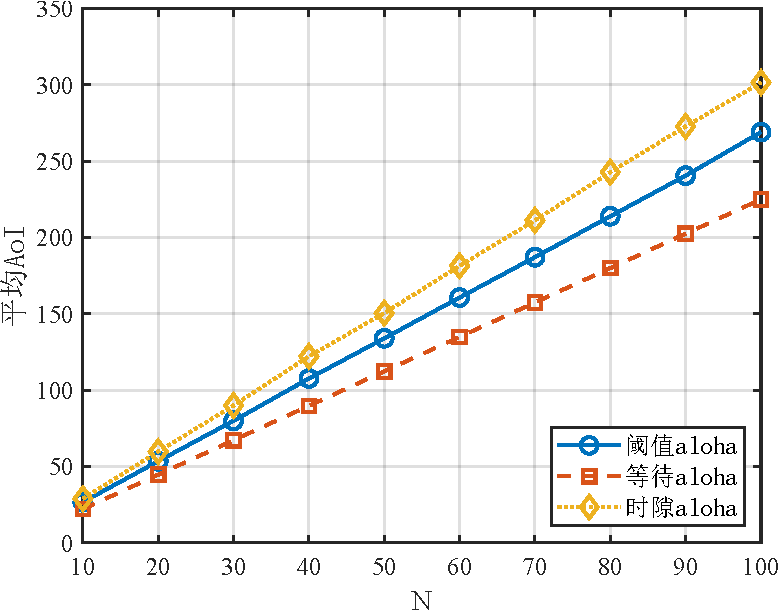
\includegraphics[width=\textwidth]{figure/cp3/不同机制的平均AoI对比.pdf}
        
        \vspace{6pt}
        {\zihao{5}\songti (a) 平均AoI理论与仿真对比}
    \end{minipage}%
    \hspace{0.06\textwidth} % 【修改2】用固定宽度替换 \hfill，控制两图中间的间隙
    % === 第二张图 (右) ===
    \begin{minipage}[t]{0.42\textwidth} % 【修改1】把 0.48 改小，例如 0.42
        \centering
        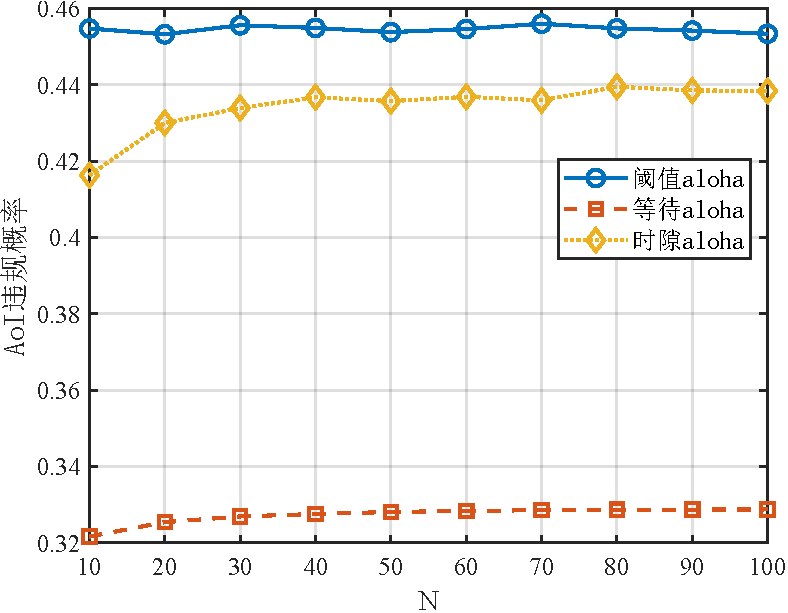
\includegraphics[width=\textwidth]{figure/cp3/不同机制的AoI违规概率对比.pdf}
        
        \vspace{6pt}
        {\zihao{5}\songti (b) AoI违规概率理论与仿真对比}
    \end{minipage}
    
    \caption{理论与仿真对比}
    \label{fig:cp3_compare} % 【修改3】\label 必须放在 \caption 之后！（建议加上 fig: 前缀方便管理）
\end{figure}

图\ref{fig:cp3_compare}的（a）展示了三种机制的平均 AoI 性能对比。在设备数量较少的网络环境中，由于信道资源相对充裕，三种机制之间的性能差距并不显著。然而，随着设备数量 $N$ 的不断攀升，等待 ALOHA 在平均 AoI 方面的优势逐渐凸显，而阈值 ALOHA 仅表现出次优的性能。这一现象的理论根源在于：阈值 ALOHA 的核心是限制“新鲜节点”的竞争，但当节点数量激增导致碰撞加剧时，节点发送成功率骤降，大量节点的 AoI 会迅速突破阈值并同时被唤醒。由于该机制缺乏碰撞后的退避惩罚，网络陷入了拥塞死锁，导致其优化机制失效。相反，等待 ALOHA 凭借碰撞后的随机退避窗口 $w$ 有效打散了高并发流量，保障了信道的稳定吞吐，从而在节点密集场景下依然能够维持较低的平均 AoI。图\ref{fig:cp3_compare}的（b）进一步展示了对工业控制至关重要的 AoI 违规概率对比。从图中可以观察到，等待 ALOHA 在抑制极端信息陈旧方面表现出了绝对的最佳性能。而令人意外的是，阈值 ALOHA 在控制违规概率方面，甚至逊色于最基础的时隙 ALOHA。这深刻地揭示了一个事实：仅仅依赖“静态阈值截断”无法应对实际网络中的复杂拥塞；而在 MAC 层引入针对碰撞的动态退避处理，对于降低 AoI 违规概率具有不可替代的显著效果。

\subsection{小结}
本章针对 mMTC 场景对信息时效性的严苛需求，指出了传统时隙 ALOHA 机制盲目竞争的弊端，并将等待机制引入到时隙 ALOHA 中，设计了等待 ALOHA 协议。该机制通过强制成功传输的节点主动退避常数时隙，为全网让渡传输机会；同时辅以碰撞后的随机退避窗口来打散拥塞。

在性能评估方面，本章利用解耦假设构建了二维马尔可夫链模型，推导出了系统的稳态自洽方程，并论证了稳态工作点的存在性与唯一性。随后，基于 AoI 演化的微观几何特征与矩匹配近似理论，成功推导出了该机制下平均 AoI 与 AoI 违规概率的闭式解析表达式。最终的仿真实验不仅证实了上述所有数学推导的极高准确性，更通过与其他 ALOHA 算法的横向对比，充分证明了等待 ALOHA 机制在抑制信息老化与降低极端时效性违规风险上的全面优越性。

